\section{Analysis}\label{sec:analysis}

% \comment{Present datasets???}

%$\datasetA = \big\{ (\vec{x}^{(1)}, y^{(1)}), \,  (\vec{x}^{(2)}, y^{(2)}), \,\dots, \, (\vec{x}^{({\npointsA})}, y^{(\npointsA)}) \big\}$ 

% \comment{Maybe write something about the codes?}


% OUTLINE:
% \begin{enumerate}
%     \item Gradient descent \begin{enumerate}
%         \item[-] OLS and Ridge on regression problem
%     \end{enumerate}
%     \item Building our FFNN
%     \item Regression problem \begin{enumerate}
%         \item[-] try different activation functions
%     \end{enumerate}
%     \item Classification problem \begin{enumerate}
%         \item[-] compare with logistic regression 
%     \end{enumerate}
% \end{enumerate}

\subsection{Gradient descent}\label{sec:analysis_SGD}


    Using the SGD algorithm, we perform an OLS regression on a dataset generated by a third order polynomial with some added noise,
    \begin{equation}
        F(x) = 2.0x + 1.7x^2 -0.40x^3 \, +\, 0.10\mathcal{N}(0, 1),
    \end{equation}
    and we consider $n=400$ data points in total, but save 20\% of these for validation. We use the Vandermonde matrix $X\in \RR[400 \cross 3]$ of row vectors $\vec{x} = (x, x^2, x^3)$ ($p=3$) so that the output becomes $\hat{y} = X\svec{\theta}$, where $\svec{\theta}\in \RR[3]$. We also scale the data via z-score normalisation. In particular, we aim to minimise the cost function in eq. \eqref{eq:linear_regression_cost_function} in $\svec{\theta}$-space with $\lambda=0$ for which we need to tune the learning rate $\eta$. We perform the same analysis using the Ridge cost function, i.e. $\lambda > 0$ in eq. \eqref{eq:linear_regression_cost_function}, but here we need to contemplate the penalty parameter $\lambda$ as well as the learning rate $\eta$.

    We want to try a variety of optimiser algorithms for different $\eta$'s. For this very simple case, after a variety of simulations, we realise a few key takeaways:
    \begin{enumerate}[label=\alph*)]
        \item\label{item:simple_a} SGD is much more robust GD.
        \item\label{item:simple_b} The effect increasing $\lambda$ has on the MSE is negligable.
        \item\label{item:simple_c} All update rules seem to find an equally good model for $\eta\in [10^{-3}, 1]$.
    \end{enumerate}
    Mainly, these things are found after performing OLS with GD, and both OLS and Ridge regression ($\lambda=0.1$) with SGD with $m=40$. More results than the ones presented in this paper can be found \href{\figureslink}{here}. Item \ref{item:simple_a} is not surprising, even though we might have exaggerated with the number of minibatches we chose. Point \ref{item:simple_b} is expected as the function is so simple, however, we noticed that the algorithms learned slightly faster. The last key point \ref{item:simple_c} indicates that the update rules are properly implemented in our code. In Figure \ref{fig:simple_reg_errors_ridge} we present the result of the Ridge regression with SGD where we used $m=40$ and $\lambda=0.1$ and stopped after 50 complete epochs. The graphs are barely distinguishable from what we got with $\lambda=0$. We see that RMSProp learns fast for small $\eta$, wheras AdaGrad seems to need a larger $\eta$ to be able to converge. With momentum, the learning requires half of the iterations needed for the plain SGD to get the same MSE, a result we repeatedly have gotten for other experiments.

    \begin{figure}
        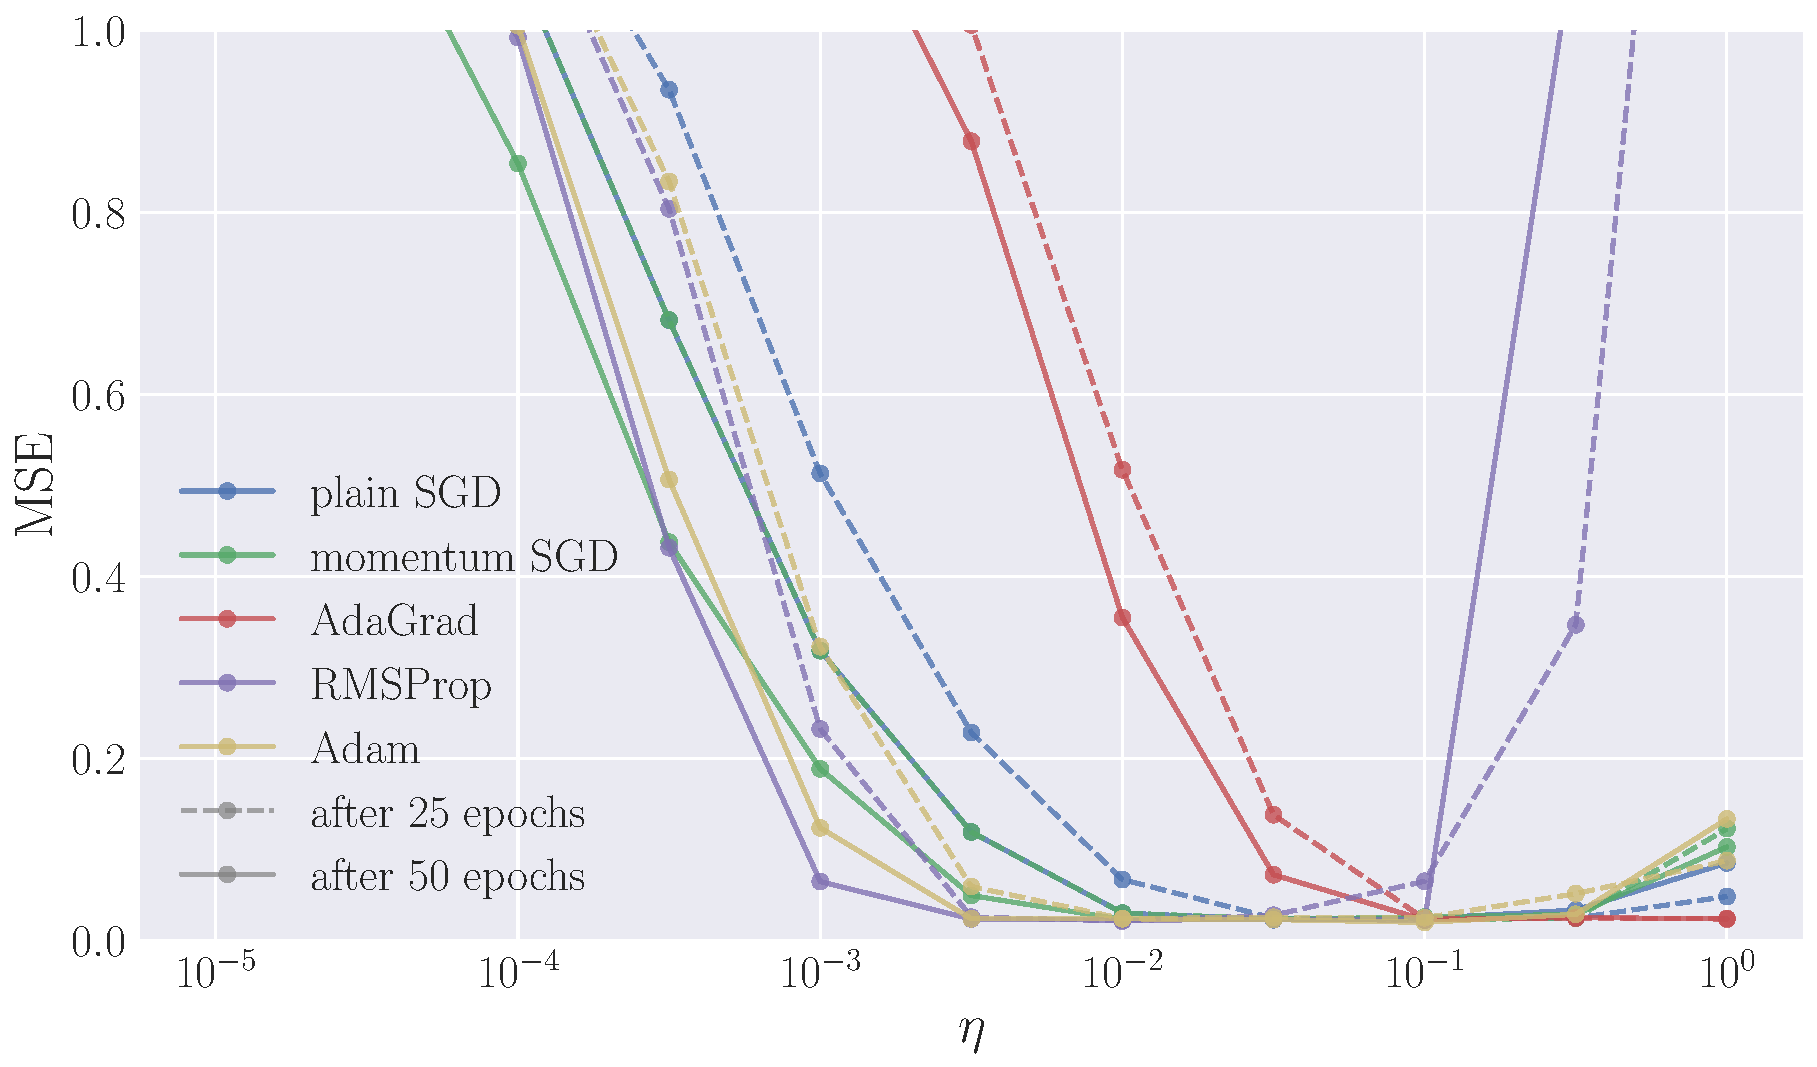
\includegraphics[width=\linewidth]{ridge_errors_gradient_descent.pdf}
        \caption{The graphs show how the test MSE evolves as the global learning rate $\eta$ increases for different update rules in the SGD algorithm. The penalty parameter is $\lambda=0.1$, and we have used $m=40$ minibatches. $\gamma=0.5$ for the momentum SGD and the other relevant hyperparameters are set to their defaults in accordance with section \ref{sec:tuning}. The dashed graphs show the MSE after 25 iterations and the solid graphs represent the MSE after 25 additional iterations. All solvers were initialised by the same random vector $\svec{\theta}_0$.}
        \label{fig:simple_reg_errors_ridge}
    \end{figure}

    We will study more thoroughly the dependencies on the number of epochs, the number of minibatches ($m$) and the penalty parameter ($\lambda$) in the NN analysis of the Franke function in section \ref{sec:analysis_NN}. 

    
\subsection{Neural network}\label{sec:analysis_NN}
    We will build our FFNN (\ref{item:prepocess}-\ref{item:optimiser}) and solve a supervised learning problem (\ref{item:train}-\ref{item:review}) using the steps listed below \citep{mhjensen}.

    \begin{enumerate}[label=(\roman*)]
        \item\label{item:prepocess} Collect and prepocess data, that is we extract 80\% of the dataset and reserve the rest for validation. The data is then scaled using standard score normalisation\footnote{Formula found in \cite{mhjensen}, or page 6 of the \projectOne-report.} with respect to the training data.
        \item\label{item:architecture} Define the model and design its architecture. In practice, this means to decide on hyperparameters of the NN such as depth ($L$) and activation function(s) ($g$).
        \item\label{item:optimiser} Choose loss function and optimiser. For regression we will use the MSE score \eqref{eq:linear_regression_cost_function} as the estimator of loss, whereas the classification problem estimates the loss according to the cross entropy \eqref{eq:logistic_regression_cost_function}. We will use SGD as optimiser, but we have various alternatives for the exact optimisation algorithm (see section \ref{sec:tuning}).
        \item\label{item:train} Train the network to find the right weights and biases.
        \item\label{item:assess} Validate model, i.e. assess model performance by applying it on the test data.
        \item\label{item:review} Adjust hyperparameters, and if necessary review the network architecture. That is to say, if the result is not satisfactory even after tuning the hyperparameters, return to step \ref{item:architecture} and start over from there. 
    \end{enumerate}

    %In practice, the steps \ref{item:architecture}-\ref{item:review} will be performed several times 
    

\subsection{Regression problem}\label{sec:analysis_regression}


    Our dataset is once again fictional as it is generated by the Franke function from \projectOne\footnote{Equation (10) in the report.} with an added noise of $0.1 \mathcal{N}(0, 1)$ for a set of coordinates in the plane. We split and standardise the $20\times 20$ data points, which concludes step \ref{item:prepocess}. 
    Eventually we want to optimise the network architecture. However, in order to begin generating result we need an initial architecture that is not too computationally expensive, but yet versatile. We initialise the network with 3 hidden layers with 15, 10, and 5 neurons each, resulting in a depth of $L=4$. The input layer has two nodes, $N_0=2$, representing the plane, whilst the output layer consist of a single node, $N_L=1$. These features of our NN are not to be changed. We begin our analysis with the sigmoid function as activation function for the hidden layers and a linear output function. We use SGD with RMSProp as our optimiser of choice, dividing the training data into $m=3$ minibatches. This concludes step \ref{item:architecture} and \ref{item:optimiser}.
    We then train our network for 250 epochs, which at this stage is a fair tradeoff between computational efficiency and fine tuning of the network. The trained model is tested against the test data and performance is recorded. 

    Now that our network is set up we are ready to tune it. The first task is to determine the hyperparameters $\eta$ and $\lambda$ given the architecture above. From \Fig{reg_eta_lambda} it is obvious that the current choice of architecture and training prefers relatively large learning rates and small regularisation parameters. The large error for smaller learning rates is most likely due the number of epoch being too small for these learning rates to find the minimum of the loss function. For now this result is satisfactory and we note the optimal parameters to be $\eta=10^{-1}$ and $\lambda=10^{-4}$. 

    Now we take a closer look at the architecture of the network and perform analysis of a model where we increase the number of hidden layers $L-1$ with a fixed, but increasing number of neurons per layer $N_l$. Note that $N_l$ is the same for $l=1,2, \dots, L-1$, and that still $N_0=2$ and $N_L=1$. \Fig{reg_layer_neuron} shows the results, where it becomes apparent that for the optimal parameters mentioned above, a network with a simple architecture (few layers and neurons) is preferred with the optimal architecture being a network with one hidden layer that contains 30 neurons. The mean squared error is steadily decreasing, and we note the current value to be $\mathrm{MSE} = 0.057$. 

    The next thing to decide is the activation function of the hidden layer. In \Fig{reg_act_epoch1000} and \Fig{reg_act_epoch} we have plotted the MSE as function of training epochs, for up to 1000 and 250 epochs respectively. For computational efficiency we want to train the network for as few epochs as necessary, but we should also check how increasing the training epochs affect the performance of the model. From these two figures we draw that the sigmoid and and hyperbolic tangent activations show the most promising results, with sigmoid being the most stable. Hence, we use sigmoid when performing the final analysis. In addition, we do not expect the model to perform significantly better if we increase the number of epochs. We also take note of the stochastic behaviour of the graphs, except for the ReLU graph. This could be since ReLU have the ability of killing neurons when its derivative is zero. 

    Having a model we need to decide on the best way of training it. \Fig{reg_minibatch_epoch} shows a heatmap of the number of epochs against the number of minibatches. Few minibatches and few epochs result in computational efficiency. However, there does not seem to be an overall preference. We therefore choose the best value of those presented and train the model over 700 epochs using 2 minibatches. 

    The final model consist of a network with one hidden layer that contains 30 neurons. The learning rate and regularisation is tuned to be $\eta=10^{-1}$ and $\lambda=10^{-4}$, where we use sigmoid as the activation function of the hidden layer. The model is trained over 700 epochs using 2 minibatches. This results in a test MSE of 0.052, which is significantly less than 0.15 as we got with normal OLS analysis in \projectOne. In order to validate our model we let the model fit a function to the original noise Franke function data. The result is shown in figure \Fig{franke}, where the data points are shown with green triangles. As is visible in the figure, the model does quite a decent job of fitting this function to the data points for the given domain. 

    \begin{figure}[h!]
        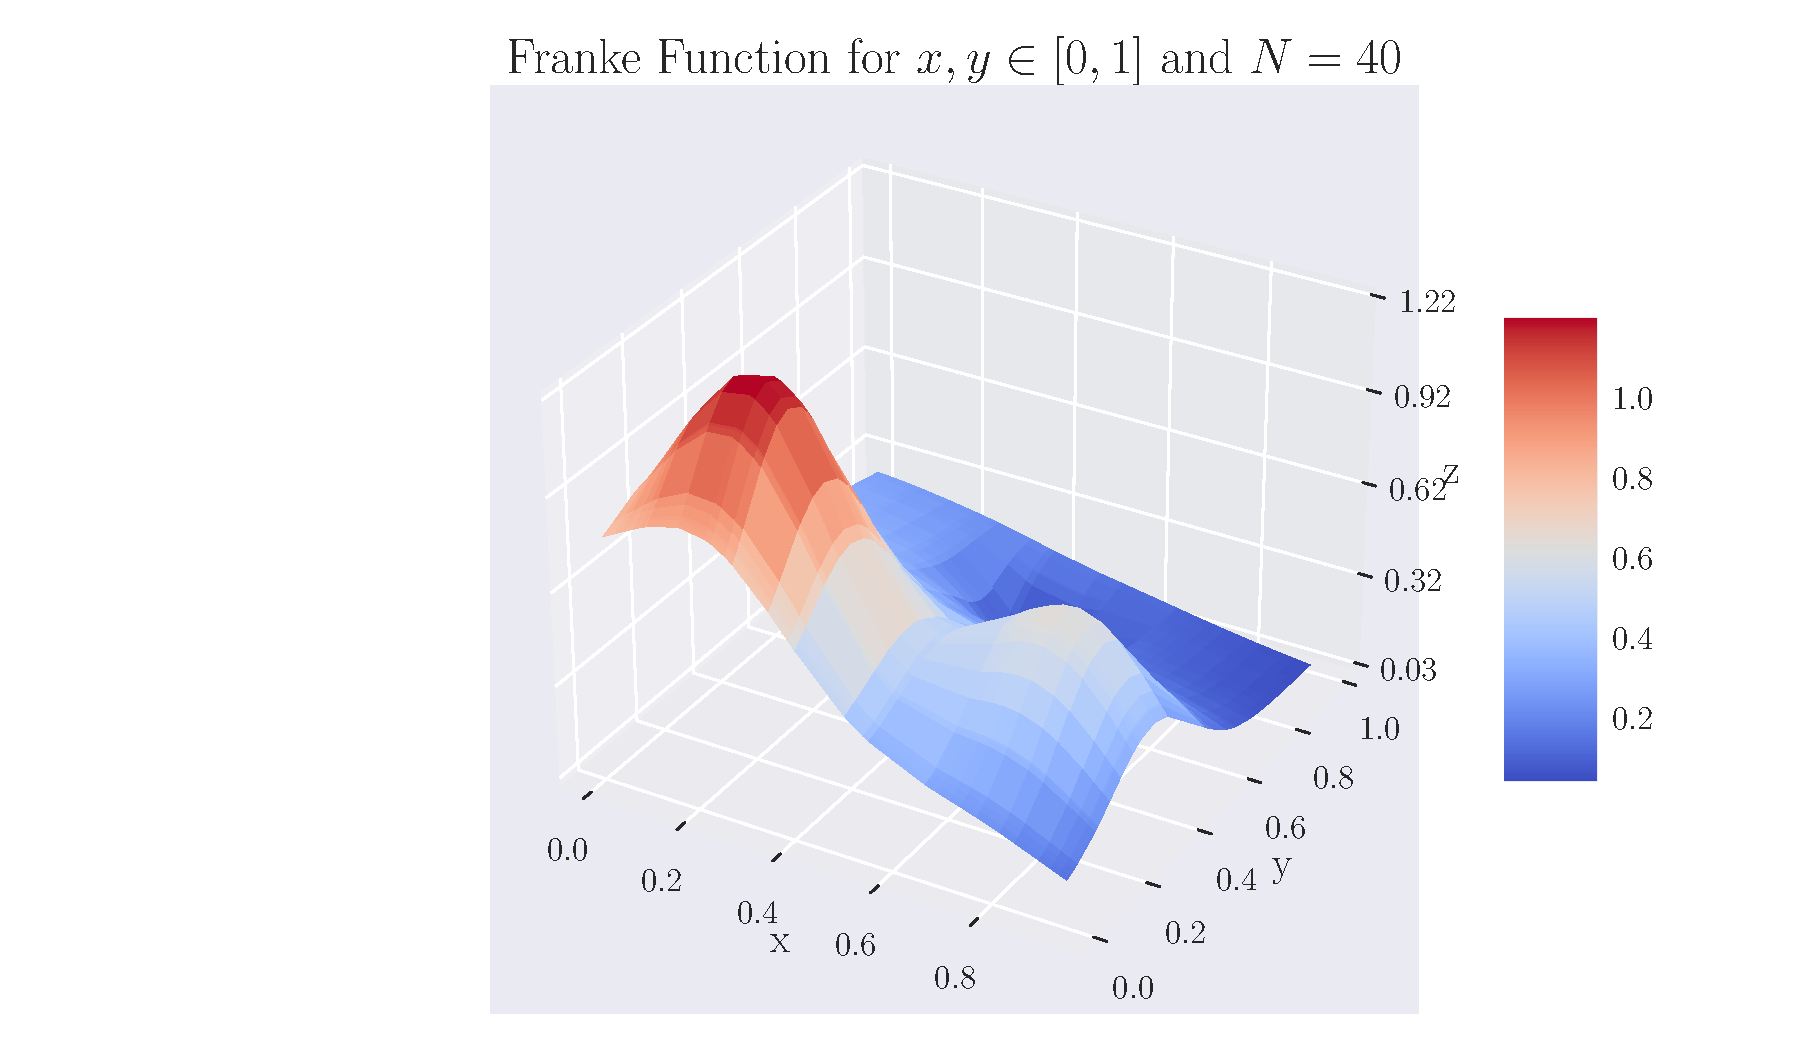
\includegraphics[width=\linewidth]{franke.pdf}
        \caption{Best fit of the Franke function (original data shown with green triangles). The model used has 1 hidden layer with 30 neurons, $\eta=10^{-1}$, $\lambda=10^{-4}$, with a sigmoid activation function trained for 700 epochs with 2 minibatches. This resulted in a test MSE of 0.052}
        \label{fig:franke}
    \end{figure}

    It is perhaps surprising that the ReLU and leaky ReLU activation functions perform so badly. One could expect that these activation function should outperform the sigmoid and hyperbolic tangent activation function. A reason for the results obtained here could very well be implementation errors in the model and initialisation. In addition, the order in which we test and decide hyperparameters should perhaps also play a role. If we revert the order and say, start with a given $\eta$ and $\lambda$ and tune the architecture before tuning the hyperparameters the result could have been different. There are numerous ways of testing and deciding on parameters for such a network, and the procedure presented here is just one of many possibilities. In the end, the MSE obtained is lower than what we found for OLS, which is a satisfactory result. Also, proposed ideal architecture is not computationally expensive and simulations are thus easy to run. 

  






\subsection{Classification problem}\label{sec:analysis_classification}
    For the classification problem we use the Wisconsin Breast Cancer dataset provided by Scikit-learn \citep{scikit-learn}. In short, this dataset consists of 569 samples, each with $p=30$ features, divided into 2 classes; those that were benign, and those that were malignant. This is thus a \textit{binary} classification problem. The major differences to our network model will be the number of input neurons, which will now be $N_0=30$, and a single output neuron with a sigmoid output function, i.e. $N_L=1, \, g_L=\sigma$. We will also use cross entropy in \Eq{logistic_regression_cost_function} as our loss function. 
    
    For comparative reasons, we perform the analysis in a similar manner as with linear regression, and we start with the same model architecture; a network with $L-1=3$ hidden layers of structure $N_1,N_2,N_3=15, 10, 5$. We minimise the loss function in the same way, using SGD with RMSProp as our chosen optimiser algorithm, starting with $m=3$ minibatches. From \Fig{class_eta_lambda} with find the optimal hyperparameters to be $\eta=10^{-3}$ and $\lambda=10^{-6}$. From \Fig{class_layer_neuron} we find the the ideal architecture, given said hyperparameters, is a network with $L-1=2$ hidden layers, each with $N_1=N_2=10$ neurons. We also note that in this case there is no significant favourisation of the simpler networks, as it was for linear regression. However, we choose the simplest one, with the highest accuracy. \Fig{class_act_epoch1000} and \Fig{class_act_epoch} show the accuracy as function of training epochs for the four different activation functions, given the above architecture. We see that the accuracy when using ReLU is close to 1, when we increase the training epochs, and we deem this to be the optimal activation function. With the above conditions, the optimal model should be trained for 900 epochs using $m=5$ according to \Fig{class_minibatch_epoch}, which gives an accuracy of 1\footnote{Given to two significant digits, which would allow for a few false predictions given the size of our dataset.}.

    The difficulties of finding an optimal model for a classification problem are similar to those of classification. The above architecture and tuning is only one of many ways of designing a model which would yield good results. It is challenging to be adamant that one model outperforms the others, since we have only tested for one, and also because the way we decide on the architecture and parameters could very well be switched around. Even for the model at hand, the heatmaps does not give a definite answer as to which set of hyperparameters or architecture is actually best, only how good they are. It is therefore wise to choose the simplest solution (most computationally efficient) that yields the most accurate result. However, the model at hand gives a descent result, and seem to work well.

\subsection{Logistic regression}\label{sec:analysis_logistic_regression}
    When performing the logistic regression analysis we notice that this is equivalent of having a neural network with no hidden layers and sigmoid as activation function. We use SGD with RMSProp as optimiser, so the only parameters we need to determine are the learning rate and regularisation. We use 250 epochs and $m=3$ minibatches. From \Fig{logistic_eta_lambda} we have that the optimal hyperparameters are $\eta=10^{-3}$ and $\lambda = 10^{-8}$. The obtained accuracy is 1\footnote{Again, to 2 significant digits, which may contain a few false predictions.}, which is satisfactory. We are thus pleased with this model and can deduce that it performs as well as the tuned neural network. 

\subsection{Closing words}\label{sec:analysis_closing_words}
    We have so far given estimates of how good our models are in terms of generalisation MSE and accuracy based on an untouched part of the dataset. There are more bulletproof ways of giving these measurements, for instance the bootstrap or cross-validation methods we discussed in \projectOne. Especially alarming are the accuracy scores of 1, which in reality is not realistic. An FFNN such as ours should not give such perfect results, however, we know that the classification dataset we use is ideal for such analyses. That is to say, there is most likely a single feature (or maybe a several few) that discloses whether a person has cancer or not. That would be plain to see if we were to make a histogram the frequency of said feature(s) where we separate the malignant cases from the benign cases and see if they overlap at all. If they do not or only a little, then this would be a very important feature. In any case, we might have benefitted especially in this case from using some resampling methods.

    In this analysis, we have favourised RMSProp as optimiser. This was due to the nice results in section \ref{sec:analysis_SGD} and because we aimed to reduce the amount of hyperparameters to tune. However, we cannot say for certain that this is the best optimiser for our loss functions. 